\chapter{Introduction}
\setheader{Introduction}
This document provides a sketch of the system that is going to be built during the context project multimedia services. The architecture of the system is explained in the form of high level components of the system. These components are split in to sub components and sub-systems.

\section{Design goals}
The following design goals will be maintained throughout the project:
\begin{itemize}

\item
\textbf{Deployability}
\\
The system will be developed in such a way that we can always deploy the most current version (Continuous Integration \cite{Duvall}).
Being able to deploy the system at any time allows us to keep the work required for a release manegable.
Because the current version should be deployable at anytime, developers are enforced to only alter the system in a non-breaking way.
Another advantage is that smaller releases\footnote{With smaller we mean releases that touches only a few lines or a few files of the codebase.} imply a lower possibility of introducing bugs.

\item
\textbf{Portability}
\\
The frontend should work on \textit{Evergreen} browsers \footnote{<<The term "evergreen browser" refers to browsers that are automatically upgraded to future versions, rather than being updated by distribution of new versions from the manufacturer, as was the case with older browsers.>> - http://www.techopedia.com/definition/31094/evergreen-browser}.
The backend should run on both Windows and Linux server environments.

\item
\textbf{Simplicity}
\\
The system will be developed with simplicity in mind.
Existing libraries and frameworks will be investigated and used if applicable, so we can focus on developing the system rather than the tools required to build the system.
This will keep our codebase relatively small and limited to the product.
% By using dependencies we do not reduce the overall complexity, in fact, these dependencies will most likely include unused funcitonality and come with a learning curve for the developers.
% ^ Not sure what to do with this line, please take into account with review - JW

\item
\textbf{Object-oriented programming}
\\
Object-oriented programming\cite{Wirfs-Brock} will be used to develop the system.
We will separate the system into subsystems and components (\glspl{Package}, \glspl{Class} and \glspl{Interface}).
This should enable code reuse and extensibility, and improve the testability of the sytem, because each component can be tested individually\cite{Binder}.

\item
\textbf{Usability}
\\
Users should be able to use Moodcat intuitively.
% Insert more

\end{itemize}

\chapter{Software architecture views}
This chapter discusses the architecture of the system.
The system is first decomposed into smaller subsystems and the dependencies between the subsystems are explained.
In the second paragraph the relation between the hardware and software of the system is elaborated.
The third paragraph illustrates the data management of the system.

\section{Subsystem decomposition}
Moodcat is subdivided into two components: the frontend and the backend service.
In this chapter we will explain how these components are composed and how they interact with each other.

\begin{figure}[h!]
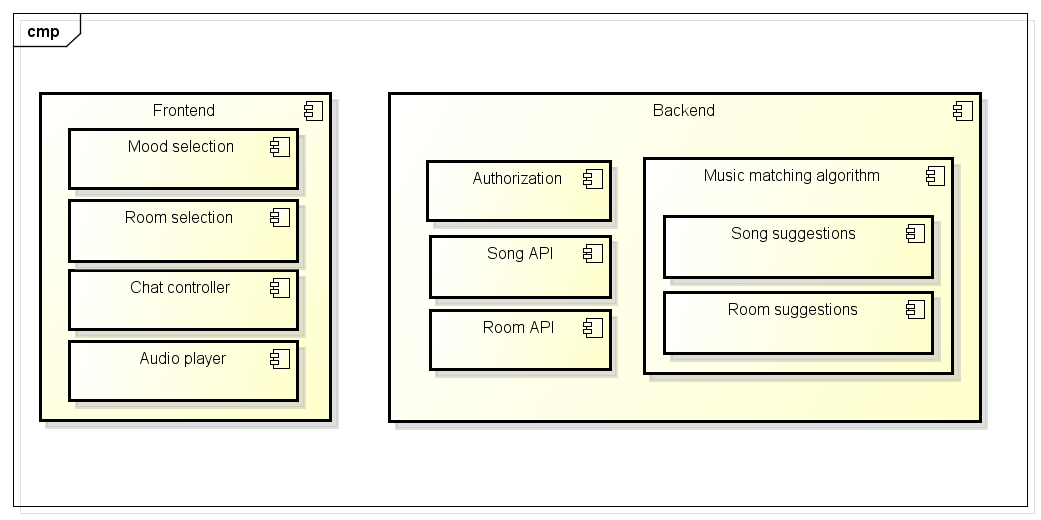
\includegraphics[scale=.6]{architectureOverview.png}
\caption{Architecture overview for Moodcat}
\label{fig:architectureOverview}
\end{figure}

\subsection{Moodcat Frontend}
The frontend will be the visible part for the listener.
After logging in to our services, the user will be able to select his mood and based on that MoodCat will provide several music listening rooms.
In these rooms the user can interact with other listeners through the chat while listening to the music.

\begin{figure}[h!]
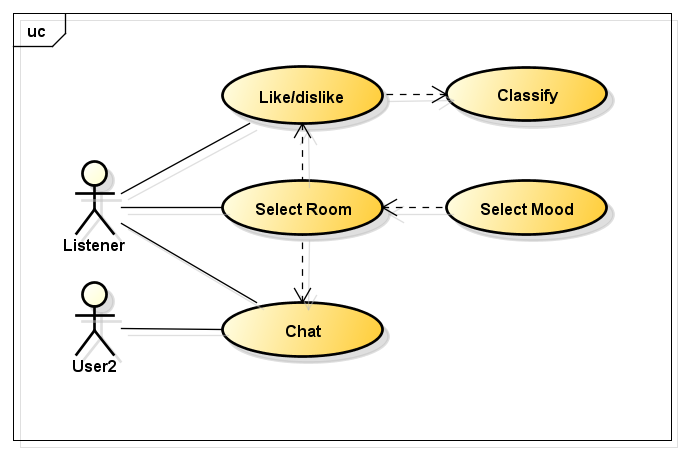
\includegraphics[scale=.4]{useCases.png}
\caption{Use case diagram for Moodcat}
\label{fig:MoodCatUseCase}
\end{figure}

\par
The MoodCat frontend will be web-based.
This allows us to support all modern devices which enables a large target audience.
We will develop the frontend using modern techniques as \Gls{HTML}\cite{HTML}, \Gls{JS} and \Gls{CSS}\cite{CSS}.
Twitter Bootstrap will be used as boilerplate for our own customized CSS thema.

\par
AngularJS\cite{AngularJS} will be used as web framework, providing us two-way data binding between the user interface and backend, and a standardized way of composing user interface controlling logic through \textit{controllers}, \textit{services} and \textit{directives}.

\par
The Object-oriented\cite{Wirfs-Brock} and Dependency Injection\cite{angularDI} driven nature of AngularJS makes it suitable for unit testing\cite{Binder}.
Testing the frontend codebase will be done using the Karma\cite{Karma} testrunner, the Jasmine\cite{Jasmine} testing framework and the PhantomJS\cite{PhantomJS} headless\footnote{JavaScript runs in browsers and the written logic needs a DOM to interact with. A headless browser does not actually render the page and is therefore much faster in intergration tests.} browser.

\subsection{Moodcat Backend}
The Moodcat backend has several subcomponents, each with their own responsibility:
\begin{itemize}
\item the \textit{Static File Server} that serves the frontend website on a webserver;
\item the \textit{REST API} which is used for communication about rooms and songs between the backend and frontend;
\item the \textit{Music matching algorithm} which is used to generate music suggestions for rooms and to find a room for a user.
\end{itemize}
In the following paragraphs we will explain the last two subcomponents.

\subsubsection{REST API}
The MoodCat REST\cite{rest} connects the frontend to the music matching algorithm.
The backend keeps track of which rooms are active and what song is currently played in the room.
Furthermore, the backend is responsible for transmitting the chat messages between the users in the room.
An example interaction between the frontend and the backend is given in \ref{fig: backendInteraction}.
% I am not so happy that we do not mention how we rely on Soundcloud for the streaming here, but I have the feeling it does not really fit here. Suggestions?

\begin{figure}[h!]
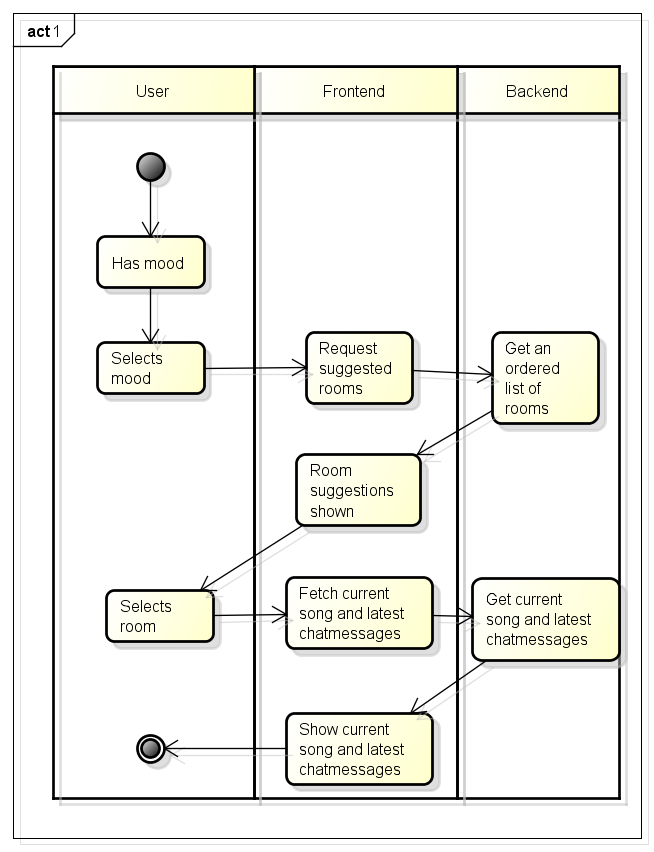
\includegraphics[scale=.4]{backendInteraction.png}
\caption{Example interaction frontend and backend}
\label{fig: backendInteraction}
\end{figure}


\par
The backend and the frontend communicate over \Gls{HTTP} requests in the \Gls{JSON} format.
% We might want to note Websockets at a later point
The REST API will be written in Java using JAX-RS and Jackson.
Jackson serializes Java objects to a JSON string based on their attributes, and vice versa: it is able to deserialize a Java object from a JSON string.
This allows us to use JSON in the frondend, which is ideal in \Gls{JS}, but use classes and objects in Java, which greatly improves the testability of the responses.
The backend will be tested using Unit tests written using JUnit and Mockito.

\subsubsection{Music matching algorithm}\label{MatchingAlgorithm}
The Music matching algorithm determines and compares moods for songs, rooms and users.
Moodcat will be developed around a learning algorithm.
This means that Moodcat will improve over time.
Default values will be determined by examining the audio features provided by our data set.
Then, through a system of user votes, the system will learn and improve over time.


\section{Hardware/software mapping}
For navigating through the user interface and posting messages in the chatroom a keyboard and mouse, or a touch screen with onscreen keyboard is required.
We will annotate our elements with proper \Gls{ARIA} accessibilty attributes so that assistive technologies, such as screen readers, will work with our service properly.

\par
Moodcat requires an audio interface to play music.
To interact with the audio interface from the browser, the Web Audio API\cite{WebAudioAPI} and NgAudio are used.
The users browser should support these techniques in order to use Moodcat.

\section{Persistent data management}
Moodcat has to handle with both song data and chatroom data.

\par
For the song we store the basic properties, like artist, song title, genre and duration.
Furthermore each song has its own valence and arousal value, which is computed and corrected by the music matching algorithm.
The algorithm uses some of the audio features of the track for the computation of the valence and arousal values, these features are stored with the song.

\par
For the chatrooms we store basic properties, the currently playing song, the room members and a chat message.

\begin{figure}[h!]
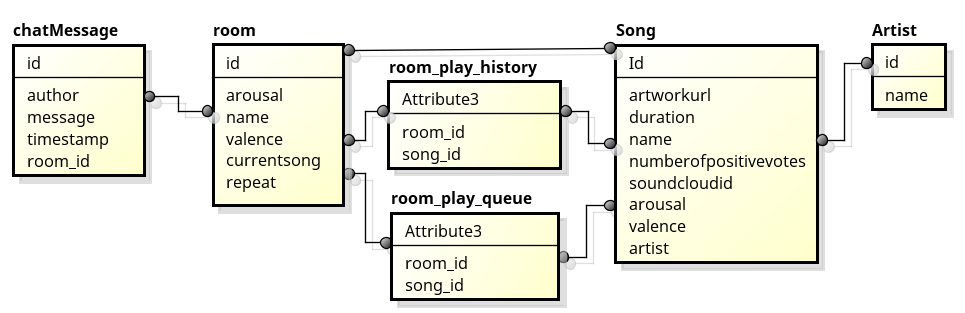
\includegraphics[scale=.4]{erDiagram.png}
\caption{ER diagram for Moodcat}
\label{fig:ER diagram of the described entities}
\end{figure}

\par
Most of the currently used data will be stored in memory, as it would be intensive to query the database for each chat message that comes in.
However, the data will eventually be persisted in a PostgreSQL\cite{PostgreSQL} \gls{RDB}.
One one hand this is because it would be impractical to store our entire dataset in memory.
% On the other hand, well the other hand is busy %
On the other hand, this is useful because then the system can continue where it has left off after a restart.

\par
We will connect our Java backend server to the PostgreSQL database using the Java Persistence API (JPA) and the Postgres JDBC driver.
The Hibernate\cite{HibernateORM} \Gls{ORM} (ORM) framework will be used to map Java class instances to tables.
QueryDSL\cite{QueryDSL} JPAQuery will be used to build \Gls{SQL} queries from Java code.
We have chosen for these techniques because they provide a nice and clean API to bind Java objects to database objects.

\section{Concurrency}
In order to scale up to thousands of connected clients, we should develop with concurrency in mind from the very first start.
Moodcat uses the Soundcloud API in order to stream media to the clients.
This means that the audio stream does not have to pass through our servers.
We do however have to handle the various API calls to interact with the backend, for example to play the next song or to broadcast a message in a room.

\par
It is important that these requests do not block each other, therefore we have chosen a servlet container that uses asynchronous sockets - which will not block if there is no data to receive yet.
Moodcat will be developed with an embedded Jetty servlet container, which uses asynchronous socket channels to connect with the clients.

\par
Besides the communication with the clients, Moodcat should also keep its algorithm (described in \ref{MatchingAlgorithm}) running in the background.
This algorithm will run in seperate threads to optimize throughput.
These seperate threads will get a specific task assigned, which has his local data to compute on.
Deadlocks will be prevented because the spawned threads will be joined before acquiring locks in synchronized statements.
This will happen when we persist the algorithm output in the database.
